%==============================================================================
%  Laatta — Architecture Specification
%  Build:  pdflatex documentation.tex   (run twice for the table of contents)
%==============================================================================
\documentclass[11pt,a4paper]{article}

\usepackage[T1]{fontenc}
\usepackage[utf8]{inputenc}
\usepackage[english]{babel}
\usepackage[a4paper,margin=25mm,headheight=15pt]{geometry}
\usepackage{amsmath}
\usepackage{graphicx}
\usepackage{booktabs}
\usepackage{tabularx}
\usepackage{fancyhdr}
\usepackage{enumitem}
\usepackage{caption}
\usepackage[hidelinks]{hyperref}

%------------------------------------------------------------------ metadata --
\newcommand{\docTitle}{Laatta --- Tile-Based GPU Architecture Specification}
\newcommand{\docID}{LAATTA-ARCH-001}
\newcommand{\docVersion}{0.3}
\newcommand{\docStatus}{Draft}
\newcommand{\docDate}{2026-09-01}
\newcommand{\docAuthor}{Jesse Oinonen}

%----------------------------------------------------------- page furniture ---
\pagestyle{fancy}
\fancyhf{}
\fancyhead[L]{\small\docID}
\fancyhead[R]{\small Version \docVersion\ --- \docStatus}
\fancyfoot[L]{\small Laatta Architecture Specification}
\fancyfoot[R]{\small Page \thepage}
\renewcommand{\headrulewidth}{0.4pt}
\renewcommand{\footrulewidth}{0.4pt}

\captionsetup{font=small,labelfont=bf}
\setlength{\parskip}{0.6em}
\setlength{\parindent}{0pt}

% Decision / assumption / question records: full text width, no narrow columns.
\newcommand{\field}[1]{\textbf{#1}\quad}
\newlist{records}{description}{1}
\setlist[records]{leftmargin=0pt,style=nextline,font=\bfseries,itemsep=0.8em}

\begin{document}

%================================================================ title page ==
\begin{titlepage}
\centering
\vspace*{2cm}

{\Huge\bfseries Laatta\par}
\vspace{0.6cm}
{\LARGE Tile-Based Deferred Rendering GPU\par}
\vspace{0.3cm}
{\Large Architecture Specification\par}

\vspace{2.5cm}

\begin{tabular}{@{}ll@{}}
\toprule
Document ID   & \docID \\
Version       & \docVersion \\
Status        & \docStatus \\
Date          & \docDate \\
Author        & \docAuthor \\
Target device & Digilent Arty Z7, Xilinx Zynq-7000 XC7Z020 \\
\bottomrule
\end{tabular}

\vspace{2.5cm}

\begin{minipage}{0.85\textwidth}
\small
\textbf{Abstract.}\quad
This document specifies the architecture of Laatta, a small tile-based deferred
rendering (TBDR) GPU implemented from scratch on FPGA. It records the
architectural decisions taken for the fixed-function pipeline together with the
measurements from the Phase~0 golden model that justify them.
\end{minipage}

\vfill
{\small Source of record: \texttt{docs/documentation.tex}}
\end{titlepage}

%========================================================== revision history ==
\section*{Revision history}
\addcontentsline{toc}{section}{Revision history}

\begin{tabularx}{\textwidth}{@{}llXl@{}}
\toprule
\textbf{Version} & \textbf{Date} & \textbf{Description} & \textbf{Author} \\
\midrule
0.1 & 2026-07-20 & Initial architecture outline: TBDR pipeline structure,
                   pixel formats, target platform. & \docAuthor \\
0.2 & 2026-07-21 & Phase~0 golden model complete. Architecture diagram updated
                   with tile buffer, tile scheduler and separate index fetch. &
                   \docAuthor \\
0.3 & 2026-09-01 & Runtime telemetry and GUI specified: \texttt{perf\_counters}
                   block, register map, snapshot semantics and panel layout. & 
                   \docAuthor \\
\bottomrule
\end{tabularx}

\newpage
\tableofcontents
\newpage
\listoffigures
\newpage

%==============================================================================
\section{Introduction}
\label{sec:intro}

Laatta is a small tile-based GPU IP implemented from scratch on FPGA, targeting
the Digilent Arty Z7 (Zynq-7000 XC7Z020). It follows the architectural
philosophy of mobile GPUs such as ARM Mali and Imagination PowerVR: tile-based
deferred rendering (TBDR).

The primary purpose of the project is to learn GPU architecture by building one
--- specifically, to understand the reasoning behind the structure of a modern
mobile GPU rather than only its implementation. The design targets low-power 2D
and light 3D rendering for embedded user interfaces such as automotive cluster
displays, industrial HMI panels and wearables, at 480p and 720p.

\subsection{How it works}

The frame is rendered in two passes. The \emph{geometry pass} transforms, clips
and culls all triangles, then bins them into small screen-space tiles, writing
the result to a parameter buffer in DRAM. The \emph{per-tile pass} then renders
one tile at a time, keeping that tile's colour and depth entirely in on-chip
BRAM for the whole time the tile is being processed. Only the finished colour is
written back to DRAM.

The consequence is that the depth buffer never reaches DRAM at all, and the
colour buffer is written exactly once, in burst-aligned blocks.

\subsection{The trade-off}

Tiling is not free. It replaces depth and colour traffic with a parameter buffer
that must be written once and read back once per tile the triangle touches, and
it adds a full frame of latency, since binning must complete before any tile can
be rasterised.

The balance therefore depends on the workload: \textbf{TBDR wins on pixels and
loses on geometry}. Measurements from the Phase~0 golden model put the saving at
22--48\,\% of total DRAM traffic compared with an immediate-mode renderer
producing pixel-identical output. For the embedded UI workload targeted here the
pixel side dominates, and tiling is clearly the right choice.

\subsection{Learning objective and what follows from it}

Data movement, not arithmetic, dominates cost in modern SoC and accelerator
design. A TBDR GPU makes that trade-off unusually concrete: tile size, on-chip
buffer budget, binning strategy and cache sizing all trade silicon area against
DRAM bandwidth, and each of them can be quantified before a line of RTL exists.
That is the reason this architecture was chosen as the vehicle for learning.

Several decisions in this document follow from that objective rather than from
product requirements:

\begin{itemize}[leftmargin=1.4em,itemsep=0.3em]
\item \textbf{Built from scratch} rather than integrating an existing GPU IP
      core. The point is the internal structure, so there is nothing to be
      gained by treating the pipeline as a black box.
\item \textbf{Implemented in phases}, each introducing one concept:
      fixed-function pipeline, then a scalar shader core, then SIMD lanes, then
      SIMT with warps, active-lane masks and divergence handling. Each phase is
      a working design, not a step towards one.
\item \textbf{A golden model precedes the RTL.} It exists to answer architecture
      questions with numbers, and doubles as the pixel-accurate verification
      reference. Every sizing decision in this document is traceable to one of
      its measurements.
\item \textbf{A deliberately modest FPGA target.} A constrained device forces
      real trade-offs; a larger one would allow decisions to be avoided rather
      than made.
\item \textbf{Simplifications are accepted where they do not affect the
      architectural lesson}, for example screen-space linear interpolation
      instead of perspective-correct, and bounding-box binning instead of exact
      edge tests. Each such simplification is stated explicitly where it occurs.
\end{itemize}

\subsection{Scope of this document}

This document covers the fixed-function pipeline: vertex transform, clipping and
culling, binning, tile buffer, rasterisation, depth test and blending.
It also covers the runtime telemetry path and the GUI that displays it
(Section~\ref{sec:gui}), since the quantities it reports are the ones the
architectural decisions were taken against.
Texturing, programmable shading, SIMD and SIMT execution are planned for later
phases and are out of scope here.

\subsection{Document conventions}

\begin{itemize}[leftmargin=1.4em,itemsep=0.2em]
\item Architectural decisions are recorded as numbered records
      \textbf{D-\textit{nn}}, each stating the decision, its rationale, the
      evidence supporting it and the blocks it affects.
\item Assumptions not yet verified against hardware are recorded as
      \textbf{A-\textit{nn}}. An assumption that turns out to be wrong
      invalidates every decision that cites it.
\item Open questions are recorded as \textbf{Q-\textit{nn}}.
\item Measurements quoted in the text always name the scene, resolution and
      configuration they were taken under.
\end{itemize}

%==============================================================================
\section{Architecture}
\label{sec:architecture}

Figure~\ref{fig:architecture} shows the pipeline, organised by the memory each
stage works against: programmable logic (FABRIC), on-chip block RAM (BRAM) and
external memory (DRAM). The geometry pass runs once per frame and ends by
writing the parameter buffer to DRAM; the per-tile pass then repeats for every
tile, reading that buffer back and keeping colour and depth on chip.

\begin{figure}[ht]
\centering
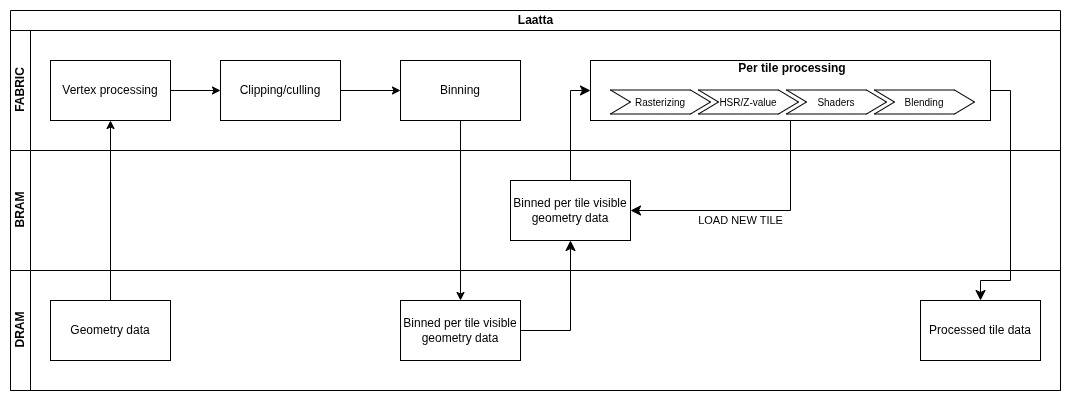
\includegraphics[width=\textwidth]{architecture.png}
\caption{Laatta pipeline.}
\label{fig:architecture}
\end{figure}

%==============================================================================
\section{Terminology}
\label{sec:terminology}

% TODO

%==============================================================================
\section{System context}
\label{sec:context}

% TODO

%==============================================================================
\section{Design decisions}
\label{sec:decisions}

Only decisions supported by Phase~0 measurements are recorded here. Remaining
decisions are added as they are taken, and existing ones are revisited when the
open assumptions of Section~\ref{sec:assumptions} are resolved.

\subsection{D-01 \quad Pixel formats}
\field{Decision.} Colour is RGBA8 (4\,B per pixel); depth is unsigned 16-bit
(2\,B per pixel), giving 6\,B per pixel of tile buffer.

\field{Rationale.} % TODO

\field{Affects.} Tile buffer sizing (D-02), tile flush, blending, framebuffer
layout.

\field{Status.} Accepted.

\subsection{D-02 \quad Tile size $32\times32$ pixels}
\field{Decision.} Tiles are $32\times32$ pixels. The tile buffer is therefore
$32\times32\times6\,\mathrm{B}=6144\,\mathrm{B}$ of BRAM.

\field{Rationale.} Tiles of $8\times8$ are disqualified outright: an 8-pixel row
is 32\,B against a 64\,B burst, so every row of the tile flush wastes half a
burst and total colour write traffic doubles. This gives a hard lower bound of
$\text{burst}/\text{bytes per pixel}=16$ pixels of tile width. Above 16 the
traffic returns are small --- 32 saves 2.9\,\% over 16, and 64 a further
1.3\,\% --- but $32\times32$ reduces the tile count from 3600 to 920 at 720p,
giving four times fewer pipeline drain and refill events at tile boundaries, a
cost the traffic model does not capture but which is real in RTL. At 6\,KB out
of roughly 630\,KB of BRAM on the XC7Z020 the on-chip cost is negligible.

\field{Evidence.} Table~\ref{tab:tile-sweep}; \texttt{model/output/sweep.csv},
\texttt{seal.obj} at $1280\times720$.

\field{Affects.} Tile buffer, binner, tile scheduler, tile flush, rasteriser.

\field{Status.} Accepted, conditional on A-01.

\subsection{D-03 \quad Post-transform vertex cache: 32 entries, FIFO}
\field{Decision.} A 32-entry post-transform vertex cache with FIFO replacement,
holding shaded vertices keyed by vertex index. Approximately 512\,B, in
distributed RAM rather than BRAM.

\field{Rationale.} Measured over the real index stream rather than assumed.
Without a cache, geometry traffic is 8.83\,MB; with 32 entries it is 2.31\,MB,
and 1.47\,MB once the asset pipeline of D-04 is applied. LRU was measured
alongside FIFO and differs by less than 0.2\,\% at every size, so the cheaper
replacement policy is chosen. Returns flatten sharply beyond 32 entries.

\field{Evidence.} Table~\ref{tab:vcache};
\texttt{model/output/vertex\_cache.csv}, \texttt{seal.obj}.

\field{Affects.} Vertex fetch, vertex shading throughput.

\field{Status.} Accepted.

\subsection{D-04 \quad Asset pipeline: triangle reorder and vertex renumbering}
\field{Decision.} Geometry is preprocessed on the host before upload: triangles
reordered for vertex-cache locality, then vertices renumbered into first-use
order and the vertex buffer permuted to match. This is a functional requirement
of the system, not an optimisation.

\field{Rationale.} Exporters emit triangles in modelling order, which caches
poorly. Applying both passes reduces geometry traffic by 37\,\% and vertex
shader invocations by 20\,\% at no hardware cost. A 32-entry cache on optimised
data (1.47\,MB) outperforms a 256-entry cache on unoptimised data (1.56\,MB) at
an eighth of the storage. Both passes are required together: reordering
triangles alone \emph{increased} DRAM bytes, because it scatters vertex fetch
addresses and destroys burst locality, and the renumbering pass restores it.

\field{Evidence.} Table~\ref{tab:vcache}, optimised columns.

\field{Affects.} Host driver, vertex fetch.

\field{Status.} Accepted.

\subsection{D-05 \quad Parameter buffer stores screen vertices, not edge
coefficients}
\field{Decision.} Each triangle occupies 40\,B in the parameter buffer: three
screen-space vertices of 12\,B each plus a 4\,B header. Tile lists hold a 4\,B
triangle index per entry with an 8\,B header per tile. Full edge-function setup
is performed in the rasteriser, per tile.

\field{Rationale.} The alternative --- performing setup before binning and
storing the coefficients --- makes each record larger, and the parameter buffer
is read once per tile the triangle touches. Since the average triangle touches
only 1.16 tiles at $32\times32$, almost no setup work is repeated, so the
smaller record wins clearly.

\field{Evidence.} Binning fan-out and parameter traffic in
Table~\ref{tab:tile-sweep}.

\field{Affects.} Binner, tile scheduler, rasteriser, parameter buffer layout.

\field{Status.} Accepted.

\subsection{D-06 \quad Bounding-box binning}
\field{Decision.} A triangle is added to every tile its screen-space bounding
box overlaps, with no exact edge test.

\field{Rationale.} Exact binning would remove some false positives, but at
$32\times32$ the average triangle already touches only 1.16 tiles, leaving
little to recover. The comparison logic would cost more than the parameter
traffic it saves.

\field{Evidence.} Table~\ref{tab:tile-sweep}, tiles-per-triangle column.

\field{Affects.} Binner.

\field{Status.} Accepted.

\subsection{D-07 \quad Rasterisation precision: 1/16 pixel, integer edge
functions}
\field{Decision.} Screen coordinates are snapped to a 1/16-pixel grid (4
fractional bits). Edge functions are exact 64-bit integer arithmetic. The fill
rule is top-left.

\field{Rationale.} Integer edge functions make coverage deterministic and
exactly reproducible between the golden model and the RTL, which is what makes
pixel-exact verification possible at all. The top-left rule ensures a pixel on
a shared edge is drawn by exactly one of the two triangles.

\field{Evidence.} Implemented in
\texttt{model/src/render/raster\_impl.h}; the tiled and immediate-mode paths
produce pixel-identical output on both test scenes.

\field{Affects.} Rasteriser, verification.

\field{Status.} Accepted.

\subsection{D-08 \quad Screen-space linear interpolation}
\field{Decision.} Vertex attributes are interpolated linearly in screen space
(affine), not perspective-correct.

\field{Rationale.} Simplification accepted for Phase~1. With Gouraud shading the
error is not visible, and it keeps the whole interpolation path in integer
arithmetic. Perspective-correct interpolation requires a per-pixel reciprocal
and becomes mandatory when texturing is added; it is therefore scheduled with
the texturing phase.

\field{Evidence.} Simplification, not a measurement. Recorded so it is not
mistaken for an oversight.

\field{Affects.} Rasteriser; revisited in Phase~3.

\field{Status.} Accepted for Phase~1.

\subsection{D-09 \quad Tile scheduler skips empty tiles}
\field{Decision.} Tiles with no triangles are not processed; their framebuffer
region is written with the clear colour without loading or rasterising
anything.

\field{Rationale.} On \texttt{seal.obj} at $640\times480$, 1063 of 1200 tiles
are empty (89\,\%). Skipping them is a basic function of the scheduler, not an
optimisation to be deferred.

\field{Evidence.} Golden model binning statistics, \texttt{seal.obj} at
$640\times480$.

\field{Affects.} Tile scheduler.

\field{Status.} Accepted.

\subsection{D-10 \quad Reset strategy: active-low, asynchronous assert,
synchronous de-assert}
\field{Decision.} The whole design uses a single active-low reset
(\texttt{rst\_n}) that is asserted asynchronously and de-asserted synchronously.
The raw reset is passed through a reset synchronizer (\texttt{rst\_n\_sync}, one
per clock domain, at the top level); every register uses the synchronized reset
in an asynchronous-reset process. This is the reset convention of an ASIC, not
the one an FPGA would choose on its own.

\field{Rationale.} The FPGA build is a prototype of an ASIC, so the RTL is kept
byte-for-byte identical to what would be taped out --- the prototype has value
only if it exercises the same logic. An ASIC uses asynchronous assert (reset
must take effect before the clock is running, at power-up) with synchronous
de-assert (releasing reset near a clock edge would otherwise let registers leave
reset on different cycles, or go metastable). Active-low matches the AXI
convention already in use (\texttt{ARESETN}). An FPGA left to its own preference
would use a synchronous, active-high reset instead, which packs and times
better.

\field{Trade-off.} The asynchronous reset costs FPGA quality-of-results: it
constrains how the tools pack registers and prevents the use of primitives that
lack an asynchronous reset (some SRL and block-RAM configurations), and the
high-fanout reset net must be placed on a global buffer. This is accepted
deliberately --- QoR of the prototype is secondary to keeping the RTL identical
to the ASIC target. Were the FPGA the product rather than a prototype, the
decision would reverse.

\field{Evidence.} Engineering convention, not a measurement.

\field{Affects.} Every sequential block; top-level reset distribution;
\texttt{rst\_n\_sync}.

\field{Status.} Accepted. (Synchronizer implementation under bring-up.)

\subsection{D-11 \quad Floating-point units: generated cores (FloPoCo) now,
own special-function unit later}
\field{Decision.} All floating-point arithmetic in the transform and lighting
datapath --- FP32 multiply, add, reciprocal, reciprocal-square-root, and later a
special-function unit for \texttt{sin}/\texttt{cos}/\texttt{exp}/\texttt{log}
--- is initially provided by FloPoCo-generated VHDL cores, instantiated behind a
stable in-house component interface (\texttt{fp\_mul}, \texttt{fp\_add},
\texttt{fp\_rsqrt}, \texttt{fp\_recip}) with a latency-agnostic valid/ready
wrapper. Hand-written equivalents are a parallel track, integrated behind the
same interface when ready, with the FloPoCo cores kept as the correctness
reference.

\field{Rationale.} The GPU pipeline can be brought up and verified without
blocking on the correctness of hand-written floating point. FloPoCo emits
synthesizable VHDL that targets both the FPGA prototype and the ASIC flow
(OpenROAD); unlike a vendor FPGA IP such as the Xilinx Floating-Point Operator,
which infers device primitives and does not pass through the open ASIC
toolchain, it therefore forces no later re-implementation to reach tape-out. Its
polynomial function evaluator is the same table-plus-polynomial structure a
from-scratch special-function unit would use, so it also serves as the golden
reference for the in-house version. Graphics tolerates a loose accuracy budget
(roughly 1\,ulp for multiply/add, several ulp for transcendentals); subnormals
are flushed to zero (FTZ) with round-to-nearest-even only, which keeps both the
generated and the hand-written units small.

\field{Trade-off.} FloPoCo uses its own internal floating-point encoding (two
exception bits above the IEEE-754 sign/exponent/mantissa); conversion happens
once at the datapath boundaries via its \texttt{InputIEEE}/\texttt{OutputIEEE}
blocks, and the FloPoCo encoding is carried through the interior. The cores
present a plain fixed-latency pipeline rather than a handshake, so each is
wrapped in the same valid/ready shell the datapath needs regardless. FloPoCo is
a command-line generator rather than an integrated IP --- a one-time setup cost.

\field{Evidence.} Engineering decision; extends the arithmetic-precision split
(floating-point transform, fixed-point rasterisation) of D-07.

\field{Affects.} \texttt{vertex\_shader} (MVP transform, normal transform,
Gouraud lighting); \texttt{clip\_cull} (perspective-divide reciprocal); any
later programmable shading. The \texttt{fp\_*} component interface.

\field{Status.} Accepted (interim). Hand-written FP / SFU track open.

%==============================================================================
\section{Micro-architecture}
\label{sec:uarch}

Blocks to be implemented in RTL for Phase~1. Each entry is completed as the
block is designed, stating its interfaces, internal state, latency, throughput
and resource usage.

\begin{table}[ht]
\centering
\begin{tabular}{@{}lll@{}}
\toprule
\textbf{Block} & \textbf{Status} & \textbf{Decisions} \\
\midrule
Geometry fetch         & Verified    & D-03, D-04 \\
\quad Index fetch      & Verified    & --- \\
\quad Vertex fetch / shading & Verified & D-03, D-04 \\
Vertex shader          & Not started & D-11 \\
Clipping / culling     & Not started & D-11 \\
Binner                 & Not started & D-05, D-06 \\
Tile scheduler         & Not started & D-02, D-09 \\
Rasteriser             & Not started & D-05, D-07, D-08 \\
HSR / depth test       & Not started & D-01 \\
Blending               & Not started & D-01 \\
Tile buffer            & Not started & D-01, D-02 \\
Tile flush             & Not started & D-01, D-02 \\
\bottomrule
\end{tabular}
\caption{Phase~1 block implementation status.}
\label{tab:blocks}
\end{table}

Each block below follows the same template, so that the blocks can be compared
and so that nothing is left unspecified by accident.

\subsection{Floating-point unit wrappers (\texttt{common/fp})}
\field{Function.} The transform and lighting datapath is built from thin VHDL
wrappers around FloPoCo-generated cores (D-11), one per operation:
\texttt{fp\_mul}, \texttt{fp\_add}, \texttt{fp\_recip} ($1/x$) and
\texttt{fp\_rsqrt} ($1/\sqrt{x}$). Each presents the same stable interface ---
\texttt{clk}, \texttt{rst\_n}, one or two 32-bit IEEE-754 operands,
\texttt{valid\_in}, a 32-bit IEEE-754 \texttt{result\_out} and
\texttt{valid\_out} --- so the FloPoCo core inside can later be swapped for a
hand-written unit without touching the datapath.

\field{Cores and latency.}
\begin{center}
\begin{tabular}{@{}lll@{}}
\toprule
Wrapper & FloPoCo core(s) & Pipeline depth (cycles) \\
\midrule
\texttt{fp\_mul}    & FPMult          & 1 \\
\texttt{fp\_add}    & FPAdd           & 3 \\
\texttt{fp\_recip}  & FPDiv           & 5 \\
\texttt{fp\_rsqrt}  & FPSqrt + FPDiv  & $6+5=11$ \\
\texttt{in\_ieee} / \texttt{out\_ieee} & InputIEEE / OutputIEEE & 0 (combinational) \\
\bottomrule
\end{tabular}
\end{center}

\field{Format and conversion.} FloPoCo uses a 34-bit internal encoding (two
exception bits above the IEEE-754 sign/exponent/mantissa). The generated
\texttt{InputIEEE}/\texttt{OutputIEEE} converters are combinational (zero
latency) and sit at the wrapper boundary: 32-bit IEEE in, 34-bit FloPoCo through
the core, 32-bit IEEE out.

\field{Valid tracking.} The cores carry data at a fixed latency but expose no
\texttt{valid}; each wrapper delays \texttt{valid\_in} by the core's pipeline
depth with a shift register (a single flop for the depth-1 multiplier). The
converters add no cycles, so the shift depth equals the core depth.

\field{Composed functions.} \texttt{fp\_recip} is \texttt{FPDiv} with the
numerator tied to the constant $1.0$; \texttt{fp\_rsqrt} chains \texttt{FPSqrt}
into \texttt{FPDiv}$(1.0,\cdot)$. The $1.0$ is hard-coded directly in the 34-bit
FloPoCo encoding (\texttt{"01"\&"0"\&"01111111"\&} zeros). \texttt{fp\_rsqrt}
keeps the FloPoCo format internally (one \texttt{InputIEEE}, one
\texttt{OutputIEEE}) rather than reusing the \texttt{fp\_recip} wrapper: separate
instances share no hardware, so nesting it would only add redundant conversions.

\field{Back-pressure.} The FloPoCo cores have no clock enable and cannot be
stalled cycle-by-cycle, so down-stream back-pressure must be absorbed at the
datapath boundaries (input gating and an output skid buffer sized to the
pipeline depth), never inside the pipeline.

\field{Status.} \texttt{fp\_mul}, \texttt{fp\_add}, \texttt{fp\_recip},
\texttt{fp\_rsqrt} implemented (interim, FloPoCo per D-11). Unit-level checking
against the C++ golden float reference is pending.

\subsection{Geometry fetch}
\field{Function.} Reads the draw descriptor from the command base
(Section~\ref{sec:memmap}), then walks the index buffer and fetches the vertex
each index points at, emitting vertices on the output stream. The index fetch
and vertex fetch stages below are internal processes of this one RTL module:
they share a single AXI4 read port and are coupled by back-pressure, so they
are not separate modules.

\field{Interfaces.} AXI4 read-only master to DRAM (\texttt{AR}/\texttt{R}
channels only; no write channels); AXI4-Stream master carrying 256-bit vertices
to the vertex shader; a \texttt{start} pulse to launch a run and
\texttt{busy}/\texttt{done} status. The descriptor address is fixed at
\texttt{CMD\_BASE}, so it is not a port; all other scene dimensions are read
from the descriptor (Table~\ref{tab:descriptor-beats}).

\field{Internal state.} Descriptor registers; current index counter; vertex
assembly register (four 64-bit beats into one 256-bit vertex).

\field{Latency and throughput.} % TODO

\field{Resources.} % TODO

\field{Related decisions.} D-03, D-04 (post-transform cache placement is open;
the baseline implementation has no cache).

\field{Status.} Verified against the block-level UVM test
(Section~\ref{sec:verification}): baseline, descriptor read plus uncached fetch,
one outstanding transaction. No post-transform cache yet (D-03).

\subsection{Geometry fetch: sequencer, AXI read channels and clock gating}

The AXI4 read handling lives inside this module rather than in a separate
\texttt{axi4\_read} block: the sequencer, the address channel and the data
channel are coupled tightly enough (shared read port, one sequencing FSM) that
splitting them added interface without value. The module is organised as one
sequencing FSM plus two channel processes.

\field{Sequencer FSM.} One FSM decides which address is issued and in what
order: descriptor first (at \texttt{CMD\_BASE}), then the index/vertex loop, an
index counter deciding when the loop ends. This FSM is the only place the read
order is defined. In the baseline it keeps a single transaction outstanding and
advances only once the current read has completed, so it never alters an
in-flight request. Multiple-outstanding pipelining --- index fetch running
ahead of vertex fetch through a FIFO --- is deferred; the index-to-vertex
address dependency means it cannot be a simple rotation and is a later
restructuring, taken only if measurement shows read latency dominates.

\field{Address channel.} \texttt{ARVALID} and the address payload
(\texttt{ARADDR}, \texttt{ARLEN}, \texttt{ARSIZE}, \texttt{ARBURST}) are asserted
together as soon as an address is ready --- \texttt{ARVALID} does not wait for
\texttt{ARREADY}, per the AXI rule --- and held stable until \texttt{ARREADY} is
seen. The address is what the slave latches at the handshake, so it must be
valid throughout the valid phase, not loaded at completion. Only after the
handshake is the next address presented, or \texttt{ARVALID} dropped if there is
none. All bursts are \texttt{INCR}; descriptor and vertex are four beats
(\texttt{ARLEN}=3, \texttt{ARSIZE}=8\,B), an index is one beat.

\field{Data channel.} \texttt{RREADY} is held asserted for the duration of a
read, so every beat is accepted as it arrives; a beat is captured when
\texttt{RVALID} and \texttt{RREADY} are both high. \texttt{RLAST} marks the last
beat and is what tells the sequencer the transaction is complete --- it replaces
the earlier \texttt{rdone} handoff. A non-\texttt{OKAY} \texttt{RRESP} raises an
error flag. Only one transaction is outstanding, so no \texttt{ARID}/\texttt{RID}
are needed; they are omitted until pipelining is added.

\field{Assembly and output granularity.} Read beats are consumed as they arrive,
each written into its slot of an assembly register --- the sequencer never
idles waiting. Data is forwarded downstream one complete unit at a time, not per
beat and not buffered until the run ends: a vertex (four 64-bit beats = one
256-bit record) is streamed out on the AXI4-Stream port the moment its fourth
beat lands, so the vertex shader transforms vertex $i$ while geometry fetch is
still fetching vertex $i{+}1$. An index arrives whole in one beat and is used
immediately to form the next vertex address; the descriptor's four beats are
assembled before \texttt{unpack\_descriptor}. Nothing waits for DONE ---
DONE only marks that the last of \texttt{index\_count} vertices has been emitted.
An index counter, incremented once per index/vertex pair and compared against
\texttt{index\_count}, ends the loop; the transition to IDLE is gated on the
final \texttt{RLAST} so the last burst is never cut short.

\field{Start / done handshake.} \texttt{start} is a single-cycle pulse from the
control register, not a held level. Capturing the pulse sets an internal
\texttt{busy} flag that stays high for the whole run and clears at DONE; a new
frame is launched by writing \texttt{start} again after the scene in DRAM has
been updated, which the module picks up because it re-reads the descriptor from
DRAM every run. A pulse arriving while \texttt{busy} is high is ignored in the
baseline; software checks \texttt{done}/\texttt{busy} before re-launching.
\texttt{busy} and \texttt{done} are exposed through the status register.

\field{Clock gating.} \texttt{busy} is also the enable for the block's clock
gate (a latch-based cell, \texttt{cg}): the read logic is unclocked until a
\texttt{start} pulse is captured and again once DONE clears \texttt{busy}. This
is coarse block-level gating on the active window, the legitimate use of clock
gating. The pulse capture and \texttt{busy} flag sit in the always-on (ungated)
domain, so the wake condition can be observed while the datapath clock is off.
Because \texttt{busy} clears only at DONE --- after the final \texttt{RLAST} ---
the clock never gates off mid-burst, which would freeze the AXI handshake and
deadlock the bus. This replaces the earlier held-\texttt{start} scheme and
removes its dependency on \texttt{start} being a level.

\field{Idle behaviour.} In IDLE / DONE only the handshake qualifiers
\texttt{ARVALID} and \texttt{RREADY} are forced to 0. The address-channel
payload is left at its last value, since AXI treats it as don't-care while
\texttt{ARVALID} is low, and clock gating freezes registers at their last
defined value rather than randomising them (the asynchronous reset of D-10
initialises them), so there is no stale-data hazard when the gated clock
restarts. DONE is entered only after the final \texttt{RLAST}, so dropping
\texttt{RREADY} there never cuts a burst short.

\field{Status.} Complete and verified. Sequencer, channel processes, start/done,
clock gate, index and vertex address generation and vertex assembly all pass the
block-level UVM test (Section~\ref{sec:verification}).

\subsection{Index fetch}
\field{Function.} % TODO

\field{Interfaces.} % TODO

\field{Internal state.} % TODO

\field{Latency and throughput.} % TODO

\field{Resources.} % TODO

\field{Related decisions.} ---

\field{Status.} Not started.

\subsection{Vertex fetch and shading}
\field{Function.} % TODO

\field{Interfaces.} % TODO

\field{Internal state.} % TODO

\field{Latency and throughput.} % TODO

\field{Resources.} % TODO

\field{Related decisions.} D-03 (32-entry FIFO post-transform cache),
D-04 (host-side index order the cache depends on).

\field{Status.} Not started.

\subsection{Tile FIFO sizing}
% TODO

%==============================================================================
\section{Memory map and data formats}
\label{sec:memmap}

The address map and buffer formats are defined by
\texttt{model/src/memory/memory\_map.h}, which is the single source of truth
and should be used to generate the RTL address constants. The tables below are
reproduced from it and must not be edited independently.

\begin{table}[ht]
\centering
\begin{tabular}{@{}lll@{}}
\toprule
\textbf{Region} & \textbf{Base} & \textbf{Contents} \\
\midrule
Command       & \texttt{0x0000\_0000} & Draw descriptor, 32\,B \\
Vertex buffer & \texttt{0x0010\_0000} & 32\,B per vertex \\
Index buffer  & \texttt{0x0080\_0000} & 32-bit indices, triangle list \\
Texture       & \texttt{0x0100\_0000} & Reserved; unused in Phase~1 \\
Parameter     & \texttt{0x0200\_0000} & Transformed triangles and tile lists \\
Framebuffer   & \texttt{0x0300\_0000} & RGBA8, row-major \\
\bottomrule
\end{tabular}
\caption{DRAM address map.}
\label{tab:memmap}
\end{table}

\subsection{Vertex format}

32\,B per vertex, chosen so that exactly two vertices fit in one 64\,B DRAM
burst: position (3 floats), normal (3 floats), texture coordinate (2 floats).

\subsection{Draw descriptor}

A 32\,B structure at the command base. The pipeline reads all scene dimensions
from it rather than from registers, so a new scene requires no RTL or register
change --- only a different descriptor in DRAM.

\begin{table}[ht]
\centering
\begin{tabular}{@{}rll@{}}
\toprule
\textbf{Offset} & \textbf{Field} & \textbf{Meaning} \\
\midrule
0  & \texttt{magic}         & \texttt{0x4C41\_4154} (``LAAT''); validates the descriptor \\
4  & \texttt{vertex\_count} & Number of vertices in the vertex buffer \\
8  & \texttt{index\_count}  & Number of indices; a multiple of three \\
12 & \texttt{vb\_base}      & Vertex buffer base address \\
16 & \texttt{ib\_base}      & Index buffer base address \\
20 & \texttt{vertex\_stride}& Bytes per vertex (32) \\
24 & \texttt{tex\_base}     & Texture base; 0 = no texture (Phase~1) \\
28 & \texttt{flags}         & Reserved \\
\bottomrule
\end{tabular}
\caption{Draw descriptor fields.}
\label{tab:descriptor}
\end{table}

\paragraph{Bit layout on a 64-bit bus.}
The descriptor is read as a single four-beat burst (\texttt{ARLEN}~=~3) from the
command base. On a 64-bit data bus each beat carries two fields: the field at
the lower offset appears on \texttt{RDATA[31:0]} and the next on
\texttt{RDATA[63:32]}. A block reading the descriptor unpacks the four beats as
follows.

\begin{table}[ht]
\centering
\begin{tabular}{@{}cll@{}}
\toprule
\textbf{Beat} & \textbf{\texttt{RDATA[31:0]}} & \textbf{\texttt{RDATA[63:32]}} \\
\midrule
0 & \texttt{magic}       & \texttt{vertex\_count} \\
1 & \texttt{index\_count}& \texttt{vb\_base} \\
2 & \texttt{ib\_base}    & \texttt{vertex\_stride} \\
3 & \texttt{tex\_base}   & \texttt{flags} \\
\bottomrule
\end{tabular}
\caption{Draw descriptor packing across the four beats of a 64-bit read burst.}
\label{tab:descriptor-beats}
\end{table}

%==============================================================================
\section{Verification}
\label{sec:verification}

Verification is at two levels: the Phase~0 golden model as the pixel-accurate
reference for the whole pipeline (Section~\ref{sec:decisions},
Appendix~\ref{app:data}), and a block-level UVM environment that checks each RTL
block against its contract as it is written.

\subsection{Block-level UVM environment}

A single UVM testbench (\texttt{ip/tb}) is reused across blocks. It provides the
agents the pipeline needs --- an AXI4 slave that models DRAM with backdoor
preload, an AXI4-Stream agent, and an optional AXI4-Lite CSR agent --- plus the
environment, base test and virtual sequence. A block is verified by adding three
files: a filelist, a block-level top that wires the DUT to the shared
interface, and a UVM test. Everything else is shared.

The block simulation is driven by \texttt{ip/scripts/sim.sh}, a lightweight
command-line flow over the Vivado xsim tools (no Vivado project):

\begin{quote}\ttfamily
scripts/sim.sh <block> [compile|elab|sim|gui|clean]
\end{quote}

\subsection{Geometry fetch --- verified}

The geometry fetch block is verified black box: the test preloads a draw
descriptor, an index buffer and a vertex buffer into the DRAM model in the
\texttt{memory\_map.h} layout, pulses \texttt{start}, and checks what comes out.
The scene uses a non-identity index list with a repeat, so index indirection and
the uncached re-fetch are both exercised. The test asserts, with a specific
\texttt{UVM\_ERROR} per failure:

\begin{itemize}[leftmargin=1.4em,itemsep=0.2em]
\item each output vertex equals \texttt{vb[indices[k]]} --- confirming descriptor
      unpack, index indirection and 4-beat vertex assembly together;
\item \texttt{TLAST} is asserted on the last vertex only;
\item the read address sequence is exactly the descriptor at \texttt{CMD\_BASE},
      then per index its 4-byte index read and the 4-beat vertex it points at,
      with the right \texttt{ARLEN}/\texttt{ARSIZE}. This check localises a
      broken address or descriptor path directly, rather than only as a wrong
      output vertex.
\end{itemize}

The test passes: all output vertices, \texttt{TLAST} and the full read sequence
match. Bring-up found and fixed three RTL faults worth recording as recurring
hazards: a missing \texttt{resize} on the index address (a 32-bit target
silently took the wrong bits of a widened \texttt{unsigned} product), a
clock-gate enable derived from the transient \texttt{start} pulse instead of a
latched active flag (the block never woke), and a re-fetch stall from a capture
flag not being cleared on the loop-back edge.

\subsection{Diagnosing a mismatch}

Against the golden model, the failure pattern localises the fault: a whole
surface wrong points at the depth sense or viewport transform; edges only at the
fill rule or subpixel snapping; individual tiles at binning or the tile flush;
colour gradients at the interpolation weights.

%==============================================================================
\section{Runtime telemetry and GUI}
\label{sec:gui}

Every sizing decision in Section~\ref{sec:decisions} was taken from a number
produced by the Phase~0 golden model, and every one of them rests on an
untimed traffic count (Section~\ref{sec:assumptions}, A-01). The GUI exists to
measure the same quantities on the running hardware and put them next to the
predicted ones. It is therefore not a decoration on top of the project but the
instrument that closes the loop between the model and the silicon: a decision
such as D-02 (tile size) or D-03 (vertex cache) is only confirmed once the
board reports the traffic the model said it would.

It has a second, more immediate use during Phase~1 bring-up. A block-level UVM
test (Section~\ref{sec:verification}) proves a block against its contract in
isolation; it says nothing about where a full frame spends its time. The
per-block activity and stall counters below are what answer that, and they
answer the one question the whole architecture is built around --- whether the
pipeline is memory-bound or compute-bound at a given tile size.

\subsection{Structure}

Telemetry is split across three levels, each doing only what it is good at.

\field{Programmable logic --- \texttt{perf\_counters}.} A counter block in the
fabric, one AXI4-Lite slave, holding free-running event counters plus a
frame-coherent snapshot register file. It only counts: an event is a single-bit
qualifier already present in the pipeline (a handshake, a \texttt{busy} flag, a
\texttt{done} pulse), and the block increments a register when it is high. There
are no dividers, no floating-point units and no timers in it.

\field{Processing system --- the telemetry agent.} Software on the Cortex-A9
that wakes on the end-of-frame interrupt, reads the snapshot as one block,
timestamps it from the PS global timer, converts counts into rates, and streams
the record to the host. It also holds the wide accumulators: the PL counters are
32-bit and the agent extends them to 64-bit across frames.

\field{Host --- the GUI.} A desktop application that receives the record stream
and draws it: current values, rolling history, and the golden-model prediction
for the same scene alongside the measured value. It reuses the existing OpenGL
viewer in \texttt{OpenGL/} with an immediate-mode UI layer, so the same binary
can display a model run and a hardware run in the same panels.

\field{Rationale for the split.} Every quantity the user actually wants is a
ratio --- frames per second, bytes per second, percent utilisation, fragments
per cycle. Ratios need division, and division in RTL costs either latency or
area for a number that changes once per frame and is read by a human. Counting
is cheap and must be in the fabric because the events only exist there;
everything else is arithmetic on twelve to forty 32-bit words per frame, which
is free on the PS. The rule for the block is therefore: \emph{the fabric counts,
software divides, the host draws.}

\field{Transport.} Records are small --- under 200\,B per frame, roughly
12\,kB/s at 60\,fps --- so the link is not a constraint. Ethernet is the
baseline because the host GUI is a separate machine; UART at 115\,200\,baud is
the fallback during early bring-up, and is sufficient if the record is sent
every $n$th frame instead of every frame.

\subsection{Quantities displayed}

Table~\ref{tab:gui-metrics} lists what the GUI shows and where each value comes
from. \emph{Counted} means a hardware counter in \texttt{perf\_counters};
\emph{derived} means computed on the PS from counted values; \emph{static} means
a read-only mirror of an RTL generic; \emph{estimated} means it is not measured
at all and is displayed as an estimate (Section~\ref{sec:gui-power}).

\begin{table}[ht]
\centering
\small
\begin{tabularx}{\textwidth}{@{}llXl@{}}
\toprule
\textbf{Quantity} & \textbf{Unit} & \textbf{Source} & \textbf{Kind} \\
\midrule
Frame rate              & frame/s      & \texttt{FRAME\_CYCLES} and $f_{\mathrm{gpu}}$ & derived \\
Frame latency           & ms           & \texttt{FRAME\_CYCLES}, \texttt{GEOM\_CYCLES}, \texttt{TILE\_CYCLES} & derived \\
Memory traffic          & B/frame      & AXI beat counters, per client & counted \\
Memory bandwidth        & MB/s         & traffic $\div$ frame time & derived \\
Triangle count          & tri/frame    & \texttt{TRI\_IN}, \texttt{TRI\_VIS}, \texttt{BIN\_ENTRIES} & counted \\
Frame count             & frames       & \texttt{FRAME\_ID} & counted \\
GPU clock               & MHz          & \texttt{REF\_CYCLES} against the PS timer & measured \\
Tile size               & px           & \texttt{CFG\_A} mirror of the RTL generic & static \\
Resolution              & px           & \texttt{CFG\_B} mirror / draw descriptor & static \\
Pipeline utilisation    & \%           & per-block active and stall counters & derived \\
Rasterisation throughput& frag/cycle, Mpix/s & \texttt{FRAG\_GEN}, \texttt{FRAG\_PASS}, \texttt{PIX\_WR} & derived \\
Power consumption       & W            & XADC sensors and an activity-weighted model & estimated \\
\bottomrule
\end{tabularx}
\caption{Quantities displayed by the GUI and how each is obtained.}
\label{tab:gui-metrics}
\end{table}

\subsection{Counter definitions}
\label{sec:gui-counters}

Each definition states what is counted, not what is displayed. Ambiguity here is
what makes a telemetry number useless later, so the counting point is named in
every case.

\field{Frame rate.} Not measured against wall time. \texttt{FRAME\_CYCLES}
counts pipeline clock cycles between consecutive end-of-frame pulses, and the
rate is $f_{\mathrm{gpu}} / \texttt{FRAME\_CYCLES}$. Deriving it from a cycle
count rather than from PS timestamps removes interrupt latency and scheduler
jitter from the number, and makes it reproducible in simulation, where wall time
has no meaning. The PS timestamp is kept in the record anyway as a cross-check;
a persistent disagreement between the two means frames are being dropped
somewhere between the PL and the display.

\field{Frame latency.} The interval from the \texttt{start} pulse that launches
a frame to the completion of the last tile flush --- the final \texttt{BVALID}
of the colour write, not the last pixel produced, since the frame is not
finished until it is in DRAM. It is reported as a total plus the split that
matters architecturally: \texttt{GEOM\_CYCLES}, the geometry pass up to the last
parameter-buffer write, and \texttt{TILE\_CYCLES}, the per-tile pass. Tiling
buys traffic at the price of a full frame of added latency
(Section~\ref{sec:intro}), and this split is where that price becomes visible.
In Phase~1 the two passes do not overlap, so frame latency and frame period are
the same number; they are counted separately regardless, because the moment the
geometry pass of frame $n{+}1$ is allowed to run against the tile pass of frame
$n$ they diverge, and a display that conflates them would silently start lying.

\field{Memory traffic.} Counted at the AXI interface as \emph{beats}, not as
bytes requested: one increment per accepted read beat
(\texttt{RVALID}\,$\land$\,\texttt{RREADY}) and per accepted write beat
(\texttt{WVALID}\,$\land$\,\texttt{WREADY}), converted to bytes by the bus width
in software. Beats are what the DRAM controller actually moves, so this is the
burst-rounded figure and is directly comparable with the byte columns of
Tables~\ref{tab:tile-sweep} and~\ref{tab:vcache}, which are burst-rounded for
the same reason. Traffic is broken out per client, using the same client
classes the golden model accounts against (\texttt{Cmd},
\texttt{IndexFetch}, \texttt{VertexFetch}, \texttt{ParamWrite},
\texttt{ParamRead}, \texttt{ColorWrite}, \texttt{Texture}), so a measured
breakdown can be placed field by field against
\texttt{model/src/memory/dram\_model.h}. The per-client split is the whole
point: a total tells you the design is memory-bound, the split tells you which
decision to revisit.

\field{Memory bandwidth.} Traffic divided by frame time, computed on the PS and
shown three ways: total MB/s, per-client MB/s, and as a percentage of the
achievable DDR bandwidth of the PS port. The last of these is only as good as
the answer to Q-01, so until that is measured the GUI shows the percentage
against the \emph{theoretical} peak and labels it as such rather than quietly
using a guess as the denominator.

\field{Triangle count.} Four counting points, because a single ``triangle
count'' hides the two ratios that matter. \texttt{TRI\_IN} counts triangles
submitted (also derivable as \texttt{index\_count}/3 from the descriptor, and
compared against it as a sanity check); \texttt{TRI\_VIS} counts those surviving
clip and back-face culling; \texttt{BIN\_ENTRIES} counts tile-list entries
written by the binner; \texttt{TRI\_RAST} counts triangles read back and set up
during the tile pass. From these the GUI shows the cull rate
$1-\texttt{TRI\_VIS}/\texttt{TRI\_IN}$ and the binning fan-out
$\texttt{BIN\_ENTRIES}/\texttt{TRI\_VIS}$, the measured counterpart of the
tiles-per-triangle column of Table~\ref{tab:tile-sweep} --- 1.16 at
$32\times32$, and the number D-05 depends on.

\field{Frame count.} A free-running 32-bit counter of end-of-frame pulses since
reset, never cleared by a snapshot. It is also the sequence number of the
telemetry record: the host detects a dropped or reordered record by a gap in it,
which matters because rates computed from a record pair straddling a gap are
wrong and would otherwise be plotted as a genuine performance event. At 60\,fps
it wraps after roughly 2.3 years of continuous running; the PS extends it to
64-bit anyway.

\field{GPU clock.} Nominally a configuration value, but displayed as a measured
one, because a wrong assumed clock silently scales every derived quantity on the
screen. \texttt{REF\_CYCLES} free-runs on the pipeline clock; the PS samples it
twice a known interval apart on its own timer and divides. The nominal value
from the clocking configuration is shown next to it, and a disagreement beyond a
small tolerance is flagged --- it means the PLL configuration is not what the
build thinks it is.

\field{Tile size.} $32\times32$ pixels per D-02, taken from the RTL generic. It
is displayed from a read-only mirror in \texttt{CFG\_A} rather than from a host
constant, so the panel reports what the loaded bitstream actually contains. The
distinction stops the most tedious class of measurement error: comparing runs
made with different bitstreams while the GUI shows the same configuration for
both.

\field{Resolution.} Handled the same way, from \texttt{CFG\_B}. Note that
resolution is not currently a field of the draw descriptor
(Table~\ref{tab:descriptor}); it is a build-time constant, so the mirror is the
only authoritative source. If resolution later becomes settable per draw, it
gains a descriptor field and the GUI reads it from there instead --- recorded as
Q-07.

\field{Pipeline utilisation.} Three counters per block, all gated by the same
frame window: \texttt{ACTIVE} (the block's \texttt{busy} is high),
\texttt{STALL\_DS} (the block holds valid output but the downstream
\texttt{tready} is low), and \texttt{STALL\_MEM} (the block is waiting on
memory --- \texttt{ARVALID} without \texttt{ARREADY}, or an accepted address
with no \texttt{RVALID} yet). Utilisation is \texttt{ACTIVE} divided by
\texttt{FRAME\_CYCLES}. The stall split is the reason for having three counters
rather than one: it attributes the idle time. A pipeline that is 40\,\% utilised
because it waits on DRAM and one that is 40\,\% utilised because a downstream
block backpressures it call for opposite fixes, and utilisation alone does not
distinguish them. The blocks instrumented in Phase~1 are geometry fetch, vertex
shader, clip/cull, binner, tile scheduler, rasteriser and tile flush.

\field{Rasterisation throughput.} \texttt{FRAG\_GEN} counts fragments the
rasteriser emits (covered samples passing the edge tests), \texttt{FRAG\_PASS}
those surviving the depth test, and \texttt{PIX\_WR} pixels written to the
framebuffer at tile flush. The GUI shows fragments per cycle --- the direct
measure of whether the rasteriser sustains its design rate --- and the effective
fill rate $\texttt{FRAG\_GEN}\times f_{\mathrm{gpu}}$ in Mpixel/s. Overdraw is
$\texttt{FRAG\_GEN}/\texttt{PIX\_WR}$, measured at 1.15 in the model on both
test scenes; Q-03 (HSR sizing) cannot be answered until this is observed on
content with real depth complexity, and this counter is what will answer it.

\subsection{Power consumption}
\label{sec:gui-power}

Power is the one quantity in Table~\ref{tab:gui-metrics} that cannot be counted,
and the panel is built to say so rather than to present a plausible number.

The Arty Z7 has no on-board current-sense rails, so board power is not readable
from the PS. The XADC does provide die temperature and the on-chip supply
voltages (\texttt{VCCINT}, \texttt{VCCAUX}, \texttt{VCCBRAM}), which are real
measurements and are displayed as such --- temperature in particular is a useful
proxy for a sustained change in activity, and a genuine indicator during long
runs.

The power figure itself is an \emph{estimate}: per-block dynamic power from the
Vivado power report at a reference activity, scaled by the activity this frame
actually had --- the same \texttt{ACTIVE} and AXI beat counters used for
utilisation --- plus the static component. It is shown with its inputs visible
(the reference report version and the scaling factors) and labelled as an
estimate everywhere it appears, never plotted on the same axis as a measured
quantity. Its intended use is comparative, not absolute: the ratio between two
configurations of the same design --- clock gating on versus off, one tile size
versus another --- is meaningful, while the absolute watt figure is not
trustworthy without a bench measurement.

A shunt or in-line USB power meter on the board supply gives a real number, but
a whole-board one that includes the PS, DDR and peripherals, so it does not
isolate the GPU either. Where such a measurement is taken it is entered into the
GUI as a separate, explicitly labelled reading rather than merged with the
estimate. Resolving this properly is Q-06.

\subsection{Register map}

\texttt{perf\_counters} is an AXI4-Lite slave in the PL register window reached
through the PS general-purpose port. It deliberately does not appear in the DRAM
address map of Table~\ref{tab:memmap}: it is a register window, not memory, and
nothing in the pipeline addresses it.

\begin{table}[ht]
\centering
\small
\begin{tabular}{@{}lll@{}}
\toprule
\textbf{Offset} & \textbf{Register} & \textbf{Contents} \\
\midrule
\texttt{0x00} & \texttt{ID}          & \texttt{0x4C41\_4154} (``LAAT''); block version in the upper half \\
\texttt{0x04} & \texttt{CFG\_A}      & Tile width, tile height, bytes per pixel (generic mirror) \\
\texttt{0x08} & \texttt{CFG\_B}      & Framebuffer width, height (generic mirror) \\
\texttt{0x0C} & \texttt{CTRL}        & Counter enable, snapshot mode, clear \\
\texttt{0x10} & \texttt{STATUS}      & Snapshot valid, overflow flags, pipeline busy \\
\texttt{0x14} & \texttt{FRAME\_ID}   & Free-running frame counter \\
\texttt{0x18} & \texttt{FRAME\_CYCLES}  & Cycles in the last frame \\
\texttt{0x1C} & \texttt{GEOM\_CYCLES}   & Cycles in the geometry pass \\
\texttt{0x20} & \texttt{TILE\_CYCLES}   & Cycles in the per-tile pass \\
\texttt{0x24} & \texttt{REF\_CYCLES}    & Free-running cycle counter, for clock measurement \\
\texttt{0x28}--\texttt{0x34} & \texttt{TRI\_*}   & \texttt{IN}, \texttt{VIS}, \texttt{BIN\_ENTRIES}, \texttt{RAST} \\
\texttt{0x38}--\texttt{0x40} & \texttt{FRAG\_*}  & \texttt{GEN}, \texttt{PASS}, \texttt{PIX\_WR} \\
\texttt{0x50}--\texttt{0x6C} & \texttt{RD\_BEATS[c]}  & Read beats per client, one word each \\
\texttt{0x70}--\texttt{0x8C} & \texttt{WR\_BEATS[c]}  & Write beats per client \\
\texttt{0x90}--\texttt{0xAC} & \texttt{ACTIVE[b]}     & Active cycles per block \\
\texttt{0xB0}--\texttt{0xCC} & \texttt{STALL\_DS[b]}  & Downstream-stall cycles per block \\
\texttt{0xD0}--\texttt{0xEC} & \texttt{STALL\_MEM[b]} & Memory-stall cycles per block \\
\bottomrule
\end{tabular}
\caption{\texttt{perf\_counters} register map. All counters are 32-bit and
read-only; \texttt{CTRL} is the only writable register.}
\label{tab:perf-regmap}
\end{table}

\subsection{Snapshot semantics}

The rule the block is built around: \emph{a record must describe exactly one
frame}. Reading counters one at a time while the pipeline runs produces a record
whose fields belong to different frames, and ratios computed from it --- a
utilisation above 100\,\%, a fan-out below one --- look like hardware faults and
have cost more debugging time in more projects than the counters ever saved.

The end-of-frame pulse therefore copies every counter into a shadow register
file in one cycle and clears the per-frame counters. The PS reads only the
shadow copy, at leisure, while the next frame is already accumulating.
\texttt{FRAME\_ID} and \texttt{REF\_CYCLES} are excluded from the clear, being
free-running by definition.

\field{Overflow.} Counters saturate rather than wrap, and set a sticky bit in
\texttt{STATUS}. A saturated counter is displayed as an explicit
``$>$'' bound in the GUI, not as its value; a wrapped one would be displayed as
a small number and believed. At 125\,MHz a 32-bit cycle counter covers 34\,s,
far beyond any single frame, so saturation in practice means the pipeline has
hung --- which is itself worth showing.

\field{Missed reads.} If the PS has not consumed a snapshot before the next
end-of-frame pulse, the new frame overwrites it and sets a
\texttt{missed} bit. The host counts these; frames whose records were lost are
gaps in \texttt{FRAME\_ID}, and the GUI breaks its history plot at a gap instead
of interpolating across it.

\subsection{Panel layout}

One window, four panels plus a status strip, arranged so the configuration that
a measurement was taken under is always on screen next to the measurement.

\begin{verbatim}
+---------------------------------------------------------------+
| frame 14 812 | 58.9 fps | 16.98 ms | 125.0 MHz | 32x32 | 720p  |
+----------------------------+----------------------------------+
| MEMORY                     | PIPELINE                          |
|  total     9.20 MB/frame   |  geom fetch  [######----]  61 %   |
|  bandwidth  542 MB/s       |     mem stall              27 %   |
|  param wr   1.35 MB   14 % |  vtx shader  [########--]  78 %   |
|  param rd   1.35 MB   14 % |  binner      [###-------]  32 %   |
|  vertex     1.47 MB   16 % |  raster      [#########-]  91 %   |
|  colour wr  3.69 MB   40 % |  tile flush  [##--------]  18 %   |
|  model says 9.20 MB   0 %  |  frag/cycle   0.87                |
+----------------------------+----------------------------------+
| GEOMETRY                   | POWER  (estimated)                |
|  submitted    55 884 tri   |  dynamic     1.4 W  (est.)        |
|  visible      31 210 tri   |  static      0.2 W  (est.)        |
|  culled          44 %      |  die temp   47.3 C  (measured)    |
|  bin entries  36 204       |  VCCINT     0.98 V  (measured)    |
|  fan-out       1.16        |                                   |
|  overdraw      1.15        |                                   |
+----------------------------+----------------------------------+
| latency: geometry 7.1 ms | tile pass 9.9 ms | frames lost 0    |
+---------------------------------------------------------------+
\end{verbatim}

Two properties of the layout are deliberate. First, the header strip carries the
configuration --- clock, tile size, resolution --- because a screenshot of the
panel has to be self-describing to be worth keeping. Second, the memory panel
shows the golden model's prediction for the same scene beside the measured
total, with the difference as a percentage; that row is the reason the GUI
exists, and putting it anywhere else would make it optional.

\field{History.} Each numeric field backs a rolling plot of the last few hundred
frames, since a frame-time or bandwidth spike is invisible in an instantaneous
reading. Records are also logged to CSV in the same column layout the model's
\texttt{sweep.csv} uses, so a hardware run and a model sweep can be compared
with the existing tooling instead of by eye.

\subsection{Cost and status}

\field{Resources.} Roughly forty 32-bit counters, their shadow copies and an
AXI4-Lite decode --- on the order of 2600 flip-flops and a few hundred LUTs, no
BRAM and no DSP. Against the XC7Z020 this is well under 3\,\% of the fabric, and
none of it is in a critical path: every counter increments off a qualifier that
already exists, and the snapshot copy is a single parallel load between frames.

\field{Effect on timing.} The counter block must not become the reason the
design misses timing. Counters are fed from registered copies of the pipeline
qualifiers rather than tapping combinational signals, accepting one cycle of
skew --- irrelevant against a frame --- in exchange for keeping the fabric fully
decoupled from the instrumentation.

\field{Related decisions.} D-02 (tile size), D-03 (vertex cache) and D-05
(parameter buffer layout) are all validated by the traffic and fan-out counters;
Q-01 (achievable DRAM bandwidth), Q-03 (HSR sizing) and Q-06 (power) are
answered, or bounded, by this section's counters.

\field{Status.} Specified; not implemented. It is scheduled after the Phase~1
pipeline produces a complete frame, since most of its counters are attached to
blocks that do not yet exist. The register map and snapshot semantics are fixed
now so that blocks can expose their qualifiers as they are written, rather than
being retrofitted.

%==============================================================================
\section{Assumptions and open issues}
\label{sec:assumptions}

\subsection{Assumptions}

An assumption that turns out to be wrong invalidates every decision that cites
it.

\begin{records}
\item[A-01 --- DRAM burst granularity is 64\,B]
Not verified against the Zynq PS DDR controller configuration. This assumption
has wider consequences than any other in the document: it sets the minimum tile
width. \emph{Affects:} D-02, and every traffic figure quoted.

\item[A-02 --- 16-bit depth is sufficient for the target content]
\emph{Affects:} D-01.

\item[A-03 --- The host performs the geometry preprocessing of D-04]
If it does not, geometry traffic rises by roughly 57\,\%. \emph{Affects:} D-03,
D-04.

\item[A-04 --- A single clock domain is sufficient for Phase~1]
\emph{Affects:} all blocks.
\end{records}

\subsection{Open questions}

\begin{records}
\item[Q-01 --- What is the real DRAM burst size and achievable bandwidth?]
Resolves A-01.
% TODO

\item[Q-02 --- How should the tile FIFO behave when a tile list exceeds its
capacity?]
On \texttt{seal.obj} at $640\times480$ with $32\times32$ tiles the average tile
list holds 94 triangles and the worst holds 4686, a spread of roughly 50 times.
The worst-case list is 187\,kB of parameter data and cannot be held on chip.
% TODO

\item[Q-03 --- How should the HSR unit be sized?]
Measured overdraw is only 1.15 on both test scenes, which are single opaque
objects and therefore not representative of a workload where HSR pays for
itself.
% TODO

\item[Q-04 --- How is the parameter buffer allocated and bounded?]
Its size depends on scene complexity, which is not known in advance.
% TODO

\item[Q-05 --- Is the framebuffer double-buffered, and what is the memory
budget?]
% TODO

\item[Q-06 --- How is power to be measured rather than estimated?]
The Arty Z7 has no on-board current-sense rails, so the power figure of
Section~\ref{sec:gui-power} is an activity-weighted estimate from a synthesis
power report, valid for comparing two configurations of the same design but not
as an absolute. An in-line measurement on the board supply gives a real number
but includes the PS, DDR and peripherals. What is needed is a defensible way to
isolate the GPU's share.
% TODO

\item[Q-07 --- Should resolution and tile size become runtime parameters?]
Both are build-time generics today, mirrored read-only into the GUI's
configuration registers (Section~\ref{sec:gui}). Making resolution runtime
settable means a new draw descriptor field (Table~\ref{tab:descriptor});
making tile size runtime settable is a far larger change, since the tile buffer
is sized from it.
% TODO
\end{records}

\subsection{Known limitations of the current measurements}

The two test scenes are single opaque objects with overdraw of 1.15, no
transparency, no textures and one draw call. They are representative of the
geometry and fill balance of simple embedded UI content, but not of a workload
with significant depth complexity. Decisions D-02 and D-03 should be re-examined
against a scene with higher overdraw before they are considered final.

%==============================================================================
\section{Roadmap}
\label{sec:roadmap}

% TODO

%==============================================================================
\appendix
\section{Measurement data}
\label{app:data}

Produced by the Phase~0 golden model. Reproduce with
\texttt{make sweep SCENE=testdata/seal.obj} in \texttt{model/}.

\begin{table}[ht]
\centering
\small
\begin{tabular}{@{}rrrrrrr@{}}
\toprule
\textbf{Tile} & \textbf{Tiles} & \textbf{BRAM} & \textbf{Entries} &
\textbf{Tiles/tri} & \textbf{Param rd} & \textbf{Total DRAM} \\
\midrule
8   & 14\,400 & 384     & 46\,283 & 1.77 & 2\,151\,680 & 13\,856\,832 \\
16  & 3\,600  & 1\,536  & 35\,251 & 1.34 & 1\,579\,904 & 9\,468\,160 \\
32  & 920     & 6\,144  & 30\,492 & 1.16 & 1\,349\,056 & 9\,196\,800 \\
64  & 240     & 24\,576 & 28\,228 & 1.08 & 1\,243\,968 & 9\,077\,248 \\
128 & 60      & 98\,304 & 27\,191 & 1.04 & 1\,196\,928 & 9\,024\,640 \\
\bottomrule
\end{tabular}
\caption{Tile size sweep. \texttt{seal.obj} at $1280\times720$, 32-entry vertex
cache, all byte figures burst-rounded. Immediate mode for the same scene:
15\,019\,584\,B.}
\label{tab:tile-sweep}
\end{table}

\begin{table}[ht]
\centering
\small
\begin{tabular}{@{}rrrrrr@{}}
\toprule
& \multicolumn{2}{c}{\textbf{Exporter order}} &
  \multicolumn{2}{c}{\textbf{Optimised (D-04)}} & \\
\cmidrule(lr){2-3}\cmidrule(lr){4-5}
\textbf{Entries} & \textbf{Hit} & \textbf{DRAM B} &
\textbf{Hit} & \textbf{DRAM B} & \textbf{Transforms} \\
\midrule
0     & 0.0\,\%   & 8\,834\,560 & 0.0\,\%   & 8\,865\,344 & 167\,652 \\
8     & 65.5\,\%  & 2\,733\,632 & 59.1\,\%  & 3\,600\,384 & 68\,569 \\
16    & 66.2\,\%  & 2\,656\,832 & 67.3\,\%  & 2\,483\,712 & 54\,757 \\
32    & 68.8\,\%  & 2\,312\,832 & 75.0\,\%  & 1\,466\,816 & 41\,884 \\
64    & 69.4\,\%  & 2\,232\,064 & 75.8\,\%  & 1\,354\,880 & 40\,516 \\
256   & 74.1\,\%  & 1\,562\,304 & 76.2\,\%  & 1\,306\,176 & 39\,940 \\
\midrule
ideal & 100\,\%   & 1\,255\,360 & 100\,\%   & 1\,255\,360 & 39\,230 \\
\bottomrule
\end{tabular}
\caption{Vertex cache measurement. \texttt{seal.obj}, 167\,652 indices, 39\,230
unique vertices, FIFO replacement. Transforms column is for the optimised
order. LRU differed from FIFO by less than 0.2\,\% at every size.}
\label{tab:vcache}
\end{table}

%==============================================================================
\section*{References}
\addcontentsline{toc}{section}{References}

% TODO

\end{document}
